\section{Study of the ternary representation}
\label{sec:ternary}

In this section, we study the ternary representation, which is the general representation with weight sharing we obtained above. We already saw that it is linear, associative and commutative.

\subsection{Genericity}

The ternary representation can represent any kind of layer. For example,
\begin{itemize}
\item To obtain a fully connected layer, one can choose $\omega$ to be of size $nm$ and $S$ the matrix of vectors that contains all possible one-hot vectors.
\item To obtain a convolutional layer, one can choose $\omega$ to be the size of the kernel. $S$ would contain one-hot vectors. A stride $> 1$ can be obtained by removing the corresponding dimensions. If the convolution is a classical convolution, or is supported by a Cayley subgraph (see \chapref{chap:2}), then $S$ would be circulant along the input neurons rank in the canonical basis.
\item To obtain a graph convolutional layer (\cite{kipf2016semi}, see description in \secref{sec:vert}), one can choose $B = 1$, $\omega = 1$, and $S$ (viewed as a matrix) to be~$\widetilde{A}$. Other variants of GCN can also be obtained, for instance to obtain Chebychev filters \citep{defferrard2016convolutional}, $S$ would be $\sum_{i=0}^k T_i(\widetilde{L})$.
\item To obtain a graph attention layer (\cite{velickovic2017graph}, see description in \secref{sec:vert}), one can concatenate $K$ graph convolutional layers, where $K$ is the number of attention heads, and with $\widetilde{A}$ filled with the learned attention coefficients. Instead of concatenation, one could also choose $\omega=K$, and given an attention head~$k$, the slices $S[k,:,:]$ would be matrices containing the learned attention coefficients.
\item Any partially connected layer with (or without) weight sharing can be obtained with appropriate construction of~$S$.
\end{itemize}

\subsection{Efficient implementation under sparse priors}

\paragraph{What is the fastest way to compute $\wideparen{\Theta S X}$ ?}
As the equation \eqref{eq:ternary} is associative and commutative, there are three ways to start to calculate it: with $\Theta S$, $SX$, or $\Theta X$, which we will call \emph{middle-stage tensors}. The computation of a middle-stage tensor is the bottleneck to compute \eqref{eq:ternary} as it imposes to compute significantly more entries than for the second tensor contraction. In \tabref{tab:mid}, we compare their shapes. We refer the reader to \tabref{tab:ind} for the denomination of the indices.

\begin{table}[H]
  \centering
\begin{tabular}{ccc}
  tensor & shape\\
  \hline
  $\Theta$ & $\omega \times N \times M$\\
  $S$ & $\omega \times n \times m$\\
  $X$ & $n \times N \times B$\\
  $\Theta S$ & $n \times m \times N \times M$\\
  $SX$ & $\omega \times m \times N \times B$\\
  $\Theta X$ & $\omega \times n \times M \times B$\\
  $\wideparen{\Theta SX}$ & $m \times M \times B$
\end{tabular}
\caption{Table of shapes}
\label{tab:mid}
\end{table}

In usual settings, we want to have $\omega \ll n$ and $\omega \ll m$, which means that we have weight kernels of small sizes (for example in the case of images, convolutional kernel are of size significantly smaller than that of the images). Also, the number of input channels $N$ and of feature maps $M$ are roughly in the same order, with $N < M$ more often than the contrary. So in practice, the size of $\Theta S$ is significantly bigger than the size of $SX$ and of $\Theta X$, and the size of $SX$ is usually the smallest.

\paragraph{How to exploit $S$ sparsity ?}
Also, in usual settings, $S$ is sparse as $S[:,i,j]$ are one-hot vectors. So computing $SX$ should be faster than computing $\Theta X$, provided we exploit the sparsity. Although $S$ is very sparse as it contains at most a fraction $\frac{1}{w}$-th of non-zero values, it is only sparse along the first rank, which makes implementation with sparse classes of common deep learning libraries use less parallelization than it can. However, we can benefit from two other sparse priors: the local receptive fields (LRF) are usualy of the same size (or at least of around the same order), and each weight is associated to one \emph{and only one} neuron of each~LRF.

So we proceed differently. The idea is to use a non-sparse tensor $X_{\LRF}$ that has a rank that indexes the LRF, and another rank that indexes elements of these LRF, in order to lower the computation to a dense matrix multiplication (or a dense tensor contraction) which is already well optimized. This approach is similar to that proposed in \cite{chellapilla2006high}, which is also exploited in the cudnn primitives~\citep{chetlur2014cudnn} to efficiently implement the classical convolution.

\paragraph{The LRF representation}
In our case, it turns out that $X_{\LRF}$ can be exactly $SX$, as given fixed~$b$,~$p$, and~$j$, $SX[:,j,p,b]$ corresponds to entries of the input signal $X[:,p,b]$ restrained to a LRF $\ccr_j$ of size~$\omega$. Therefore,
\begin{gather}
\exists \LRF_j = [i_1, \ldots, i_\omega]~\st SX[:,j,p,b] = X[\LRF_j, p, b]
\label{eq:R}
\end{gather}
The elements of $\LRF_j$ can be found by doing a lookup in the one-hot vectors of~$S$, provided each kernel weight occurs exactly once in each LRF. We have:
\begin{gather}
R_j[k] = i_k~\st S[:,i_k,j][k] = 1
\end{gather}
This lookup needs not be computed each time and can be done beforehand. Finally, if we define $\LRF = [\LRF_1, \ldots, \LRF_m]$, \eqref{eq:R} gives:
\begin{gather}
SX = X[\LRF, :, :]
\label{eq:LRF}
\end{gather}
The equation \eqref{eq:LRF} is computed with only $\omega \times m$ assignations and can be simply implemented with automatic differentiation in commonly used deep learning libraries.

\paragraph{Benchmarks}
To support our theoretical analysis, we benchmark three methods for computing the tensor contraction $SX$:
\begin{itemize}
  \item naively using dense multiplication,
  \item using sparse classes of deep learning libraries,
  \item using the LRF based method we described above.
\end{itemize}

We run the benchmarks under the assumptions that $S[:,i,j]$ are one-hot vectors, and that a weight occurs exactly once in each LRF (as it is the case for convolutions supported by a Cayley subgraph). For each method, we make $100$ runs of computations of $SX$, with $S$ and $X$ being randomly generated according to the assumptions. In \tabref{tab:ben}, we report the mean times. The values of the hyperparameters were each time $n = m = N = M = B = 256$, and $\omega = 4$. The computations were done on graphical processing units (GPU)\footnote{The GPU was an Nvidia Geforce GTX1060, the CPU was an Intel Xeon E5-1630v4 at 3.70GHz with 4 cores.}.

% \begin{table}[H]
%   \centering
% \begin{tabular}{lcc}
%   Method & No parallelization & Wall clock\\
%   \hline
%   Naive & 5650~ms & 950~ms\\
%   Sparse & \textbf{521}~ms & 413~ms\\
%   LRF & 1090~ms & \textbf{365}~ms
% \end{tabular}
% \caption{Benchmark mean times}
% \label{tab:ben}
% \end{table}
\begin{table}[H]
  \centering
\begin{tabular}{lc}
  Method & Mean time\\
  \hline
  Naive & 950~ms\\
  Sparse & 413~ms\\
  LRF & \textbf{365}~ms
\end{tabular}
\caption{Benchmark (100 runs each)}
\label{tab:ben}
\end{table}

We observe that the LRF method is faster, since the sparse implementation isn't optimized for this use case.

\subsection{Influence of symmetries}
\label{sec:sym}

In the case of images, or other signals over a grid, the grid structure of the domain defines the weight sharing scheme $S$ of the convolution operation. For example, for a layer $\cl : X  \mapsto Y = h(\wideparen{\Theta S X})$, and given fixed $b,p,q$, the classical convolution can be rewritten as
\begin{align}
y[j] &= h\left(\displaystyle \sum_{k=1}^{\omega} \theta[k] \h{2} \sum_{i=1}^n S[k,i,j] \h{2} x[i] \right)\\
&= h\left(\displaystyle \sum_{k=1}^{\omega} \theta[k] \h{2} x_{\LRF}[k,j] \right) \label{eq:rewr}
\end{align}
Where $x_{\LRF}[k,j]$ can be obtained by matching \eqref{eq:rewr} with the expression given by the definition (see \defref{def:conv}). So, $S[k,:,j]$ is a one-hot vector that specifies which input neuron in the LRF of $y$ is associated with the $k$-th kernel weight, and the index of the $1$ is determined by $x_{\LRF}[k,j]$.

That is to say, in the ternary representation, $\Theta$ captures the information the layer has learnt, whereas $S$ captures how the layer exploits the symmetries of the input domain.

\paragraph{Visual construction}
Visually, constructing $S$ amounts to move a rectangular grid over the pixel domain, as depicted on \figref{fig:rect} where each point represents the center of a pixel, and the moving rectangle represents the LRF of its center $j$. Each of its squares represents a kernel weight $\theta[k]$ which are associated with the pixel $x_{\LRF}[k,j]$ that falls in it.

\begin{figure}[h!t]
      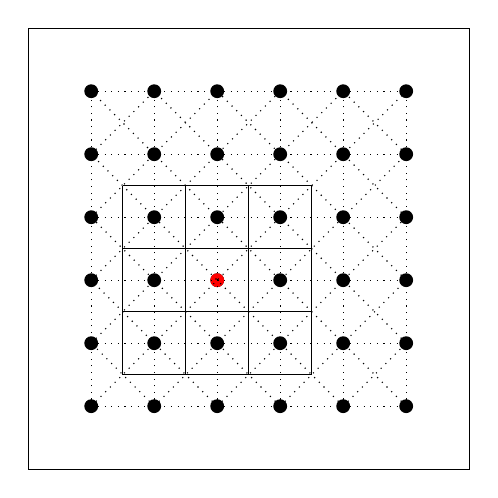
\begin{tikzpicture}[scale=0.8]%[scale=0.75]
        \tikzstyle{every node}= [circle,fill=black, minimum size= 5pt,inner sep=0pt];
          \foreach \x in {1,2,3,4,5,6}{
            \foreach \y in {1,2,3,4,5,6}{
              \node(\x\y) at (\x,\y) {};
            }
          }
          \node(33)[circle,fill=red] at (3,3) {};
          \foreach \x in {1.5,2.5,3.5,4.5}{
            \path[thin]
            (\x,1.5) edge (\x,4.5)
            (1.5,\x) edge (4.5,\x);
          }

          %\draw[ultra thin] (1,6.17) edge[<->] (2,6.17);
          %\node[draw=none,fill=none] at (1.5,6.3) {\scriptsize{$\mu$}};

          \foreach \x in {1,2,3,4,5,6}{
            \draw[dotted,thin] (1,\x) -- (6,\x);
            \draw[dotted,thin] (\x,1) -- (\x,6);
          }

          \foreach \x in {1,2,3,4,5}{
            \draw[dotted,thin] (1,\x) -- (7-\x,6);
            \draw[dotted,thin] (6,\x) -- (\x,6);
          }

          \foreach \x in {2,3,4,5}{
            \draw[dotted,thin] (\x,1) -- (6,7-\x);
            \draw[dotted,thin] (7-\x,1) -- (1,7-\x);
          }

          \draw (0,0) rectangle (7,7);

          %\node[draw=none,fill=none] at (0.9,0.4) {$S=\bbe$};
      \end{tikzpicture}
      \caption{Weight assignement of convolutions on pixel domains}
      \label{fig:rect}
\end{figure}

The case of images is very regular, in the sense that every pixels are regularly spaced out, so that obtained $S$ is circulant along its last two ranks. This is a consequence of the translational symmetries of the input domain, which underly the definition of the convolution, as seen in \chapref{chap:2}.
\begin{itemize}
\item What happens if we loose these symmetries?
\end{itemize}

To answer this question, we make the following experiment~\citep{vialatte2016generalizing}:
\begin{enumerate}
\item We distort the domain by moving the pixels randomly. The radial displacement is uniformly random with the angle, and its radius follows a gaussian distribution~$\cn(0,\sigma)$.
\item Then we compare performances of shallow CNNs expressed under the ternary representation, for which $S$ is constructed similarly than with the above visual construction, for different values of~$\sigma$.
\end{enumerate}

The visual construction of $S$ on distorded domain is depicted by \figref{fig:distrect}.

\begin{figure}[H]
      \begin{tikzpicture}[scale=1.5825]%[scale=1.055]
        \pgfmathsetseed{5}
        \tikzstyle{every node}= [circle,fill=black, minimum size= 5pt,inner sep=0pt];
        \foreach \x in {1,2,3,4}{
          \foreach \y in {1,2,3,4}{
            \node(\x\y) at (\x+0.5*rand,\y+0.5*rand) {};
          }
        }
        \foreach \y in {1,2,3,4}{
            \node(3\y) at (3+0.5*rand,3+0.5*rand) {};
        }
        \node(33)[circle,fill=red] at (2.5,2.5) {};
        \foreach \x in {1.6,2.2,2.8,3.4}{
          \path[dashed]
          (\x,1.6) edge (\x,3.4)
          (1.6,\x) edge (3.4,\x);
        }

        %\draw[ultra thin] (1.6,1.45) edge[<->] (3.4,1.45);
        %\draw[ultra thin] (2.8,3.55) edge[<->] (3.4,3.55);
        %\node[draw=none,fill=none] at (2.5,1.25) {\scriptsize{$(2p+1)\mu$}};
        %\node[draw=none,fill=none] at (3.15,3.7) {\scriptsize{$\mu$}};

        \draw (0,0) rectangle (5,5);
        %\node[draw=none,fill=none] at (0.7,0.3) {$S=\bbe$};
      \end{tikzpicture}
      \caption{\etodo}
      \label{fig:distrect}
\end{figure}

We run a classification task with standard hyperparameters on a toy dataset (we used MNIST, \cite{lecun1998mnist}). The results are reported in \figref{fig:expres}.

\begin{figure}[h!tb]
  \centering
  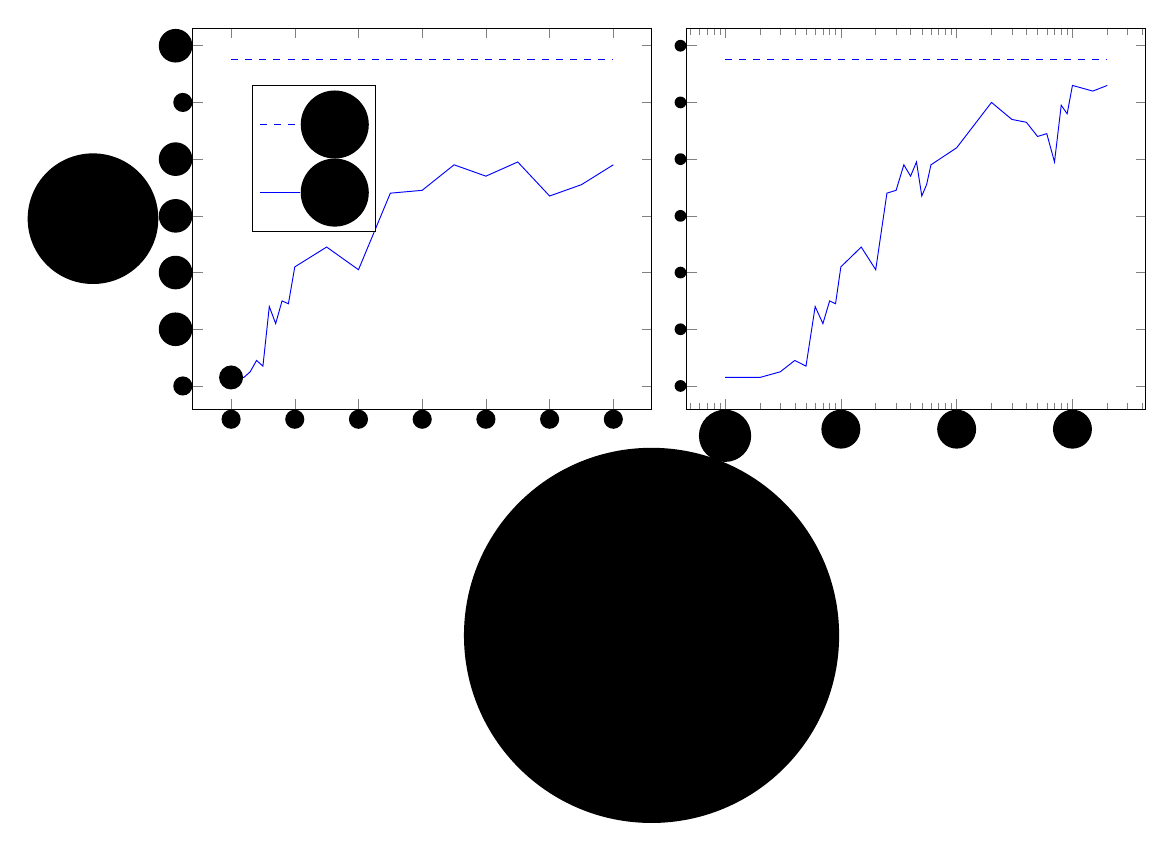
\begin{tikzpicture}[scale=0.85]
    \begin{axis}[xlabel=$\sigma$ (in unit of initial pixel separation), ylabel=Error (in \%),
      legend style={at={(0.4,0.85)}, anchor=north east},
      x label style={at={(axis description cs:1,-0.1)},anchor=north}]

      \addplot[color=blue,dashed,mark=.] coordinates {
        (0.0, 2.15) (6.0, 2.15)
      };

      \addplot[color=blue,mark=.] coordinates {
      (0.0, 1.03)
      (0.1, 1.03)
      (0.2, 1.03)
      (0.3, 1.05)
      (0.4, 1.09)
      (0.5, 1.07)
      (0.6, 1.28)
      (0.7, 1.22)
      (0.8, 1.30)
      (0.9, 1.29)
      (1.0, 1.42)
      (1.5, 1.49)
      (2.0, 1.41)
      (2.5, 1.68)
      (3.0, 1.69)
      (3.5, 1.78)
      (4.0, 1.74)
      (4.5, 1.79)
      (5.0, 1.67)
      (5.5, 1.71)
      (6.0, 1.78)
      };

      \node at (0.0, 1.03) {+};
      %\node at (0.0, 1.10) {\scriptsize{CNN}};

      \legend{MLP, CNN}
    \end{axis}

    \begin{scope}[xshift = 210pt]
      \begin{semilogxaxis}[yticklabels={,,}]

        %\node at (0.1, 1.49) {+};

        \addplot[color=blue,mark=.] coordinates {
        (0.0, 1.03)
        (0.1, 1.03)
        (0.2, 1.03)
        (0.3, 1.05)
        (0.4, 1.09)
        (0.5, 1.07)
        (0.6, 1.28)
        (0.7, 1.22)
        (0.8, 1.30)
        (0.9, 1.29)
        (1.0, 1.42)
        (1.5, 1.49)
        (2.0, 1.41)
        (2.5, 1.68)
        (3.0, 1.69)
        (3.5, 1.78)
        (4.0, 1.74)
        (4.5, 1.79)
        (5.0, 1.67)
        (5.5, 1.71)
        (6.0, 1.78)
        (10.0, 1.84)
        (20.0, 2.00)
        (30.0, 1.94)
        (40.0, 1.93)
        (50.0, 1.88)
        (60.0, 1.89)
        (70.0, 1.79)
        %(75.0, 1.91)
        (80.0, 1.99)
        (90.0, 1.96)
        (100.0, 2.06)
        (150.0, 2.04)
        (200.0, 2.06)
        };

        \addplot[color=blue,dashed,mark=.] coordinates { 
        (0.0, 2.15)
        (0.1, 2.15)
        (200.0, 2.15)
        };

      \end{semilogxaxis}
    \end{scope}

  \end{tikzpicture}
  \caption{Error in function of the standard deviation $\sigma$, for generalized CNNs and an MLP, each with $500$ weights.}
  \label{fig:expres}
\end{figure}

The bigger is $\sigma$, the less accurate are the symmetries of the input domain, up to a point where the ternary representation becomes almost equivalent to a dense layer. The results illustrate nicely this evolution, and stress out the importance of trying to leverage symmetries when defining new convolutions.

Moreover, they indicate that the ternary representation also allows to improve performances compared to using dense layers, providing we are able to prototype a relevant weight sharing scheme $S$ to exploit symmetries.

% \subsection{Randomly assigning weights}

% As we saw, the weight sharing scheme $S$ labels the propagation. In the case of datasets with known symmetries like image datasets, we saw in the previous section that it is best to do this labelling with respect to these symmetries. In the other case, when the symmerties are unknown, we can try to assign weights randomly. The idea is that, for each couple $(p,q)$ of input channel and output feature map, we randomly assign weights from the kernel $\Theta[:,p,q]$ to the propagation. Then, after propagation, we follow with a FC layer on the feature\'s dimension, as if we were learning which features have learnt the best representation in the previous layer. 

\subsection{Semi-supervised node classification}

When transposing the problem to the task of semi-supervised node classification, a ternary layer can be understand as a multi-head GCN \citep{kipf2016semi}, for which each head may correspond to a different graph.

\todo{include an experiment if time ? ie with sampled graph for each head}

% \todo{transpose, w=1}
% kipf is ternary rep but w = 1
% Idea: multiple graphs, each graph is a w
% Redo kipf experiments with directed graph, one w for the digraph, and another w for its transpose

